
\documentclass[12pt]{article}
\usepackage{enumitem}
\usepackage{mathtools}
\usepackage{amsthm}
\usepackage{graphicx}
\graphicspath{ {images/} }
\begin{document}

\title{Assignment 1}
\author{Darwin Ding}
\maketitle

\section*{Exercise 1.3}
\begin{enumerate}[label=(\alph*)]
	\item We know that $y(t) = sign(w^T(t) x(t))$. If $x(t)$ is misclassified by $w(t)$, then $y(t)$ will be opposite in sign from $sign(w^T x)$ (and therefore will be opposite in sign from $w^T x$). Therefore, $w^T(t) x(t) y(t)$ must be negative because of this difference in signs.
	\item $w^T(t) x(t) > 0$, then $y(t) = -1$ for that example t, where t is misclassified. \\ By definition: $w(t) = [w_0, w_1, w_2, ...]$ and $x = [x_0, x_1, x_2, ...]$
	\\
	\\ Therefore, using the update formula: 
	\begin{gather*}
		w(t+1) = [w_0 - x_0, w_1 - x_1, w_2 - x_2, ...]
		\\ w^T(t+1) x(t) = x_0 * (w_0 - x_0) + x_1 * (w_1 - x_1) + x_2 * (w_2 - x_2)... 
		\\ = x_0 * w_0 - x_0^2 + x_1 * w_1 - x_1^2 + x_2 * w_2 - x_2^2 + ... 
		\\ = w^T(t) x(t) - x_0^2 - x_1^2 - x_2^2 - x_3^2 - ...
	\end{gather*}
	This is strictly smaller in magnitude than $w^T(t)x(t)$, as all of the (possibly negative) data-values have been squared. This new value at t+1 may even be opposite in sign from t.
	\\ \\ If $w^T(t+1) x(t)$ did not change signs and is simply smaller in magnitude, then $y(t) w^T(t+1) x(t)$ will be negative, but smaller in magnitude. This follows the inequality, because a lesser in magnitude negative number is greater than a larger in magnitude negative number.
	\\ \\ If $w^T(t+1) x(t)$ changed signs, then $y(t)$ is the same sign as $w^T(t+1) x(t)$ and the resulting product is positive. This is by definition larger than any negative number, and this also resolves the inequality.
	\\ \\ Note that the caveat that these may be equal if all the x-values are 0 does not actually apply, since before applying the PLA algorithm we strictly appended a 1 value to the beginning of each data vector. Thus, no data-vector can be all 0s and $y(t)w^T(t+1)x(t) > y(t)w^Tx(t)$.
	\\ \\ Also note that by reversing the signs, the above can be also applied to the case where $w^T(t) x(t) < 0$, where $y(t) = 1$.
	\item If the above iteration corrects the value, by definition we have gotten better at classifying x(t) (because we had not classified it correctly before and now we are doing it correctly). If it does not correct the value outright, we can continue running the same algorithm on the same data point until it does correct it. We know it will correct it eventually because the inequality is strictly greater than, not greater than or equals.
\end{enumerate}

\section*{Exercise 1.5}
\begin{enumerate}[label=(\alph*)]
	\item \textbf{Learning} approach. Biology is one of the least understood fields out there. Pretty much everything that is known about the medical field has been determined through careful trial and error, and it's very difficult to totally understand how a body will react to any random new medical test. As a result, it's best to learn from data here.
	\item \textbf{Design} approach. Determining whether a number is prime or not has no hidden unknown function that learning from data could uncover. We could simply search for a factor of the number between 1 and itself exclusive to determine its primality.
	\item \textbf{Learning} approach. Fraud detection is an incredibly complicated task. A credit card account could have a million different values that could possibly tie into determining whether a specific purchase is fraudulent, including past purchases, location of purchase, time of purchase and cost, and so forth.
	\item \textbf{Design} approach. Although real life physics are a little more complicated than idealized physics, we can do very strong approximations for projectile motion using simple physics equations. We can measure air resistance, whether an object is in free-fall or not, and use Newtonian mechanics to get very close to actual values.
	\item \textbf{Design} approach. Although traffic theory is very complicated, it is a pretty well explored field. Correctly implementing the lights around any specific intersection just comes down to following the rules well-known by traffic engineers.
\end{enumerate}

\section*{Exercise 1.6}
\begin{enumerate}[label=(\alph*)]
	\item \textbf{Supervised} learning. Sites like this probably has a rating system where people rate the books they've bought. Therefore there's a whole flood of data that involves whether a person likes or dislikes various books. This is similar to the Netflix example with movie recommendations.
	\item \textbf{Reinforcement} learning. Tic-tac-toe is a game that can be solved algorithmically due to its simplicity, but if you're going to be learning from data it's very easy to implement the game logic and let the learning algorithm fail spectacularly.
	\item \textbf{Unsupervised} learning. Here we have a lot of complex data points (movie ratings, genres, lead actors, etc.) and we're trying to find relationships within the data.
	\item \textbf{Supervised} learning. There is a whole plethora of information on the internet about how to properly play various instruments, so a machine would likely go down the same routes as a human would (for instance with piano, how long to hold down each key and how hard to strike them for various dynamics).
	\item \textbf{Supervised} learning. This is similar to the credit problem. Banks have tons of existing data on customers with varying credit limits and backgrounds, and data on how much money they made off of those limits.
\end{enumerate}

\section*{Exercise 1.7}
\begin{enumerate}[label=(\alph*)]
	\item Picking only 1 (black) matches the data set the best, so this learning algorithm will do that.
	\begin{enumerate}
		\item Agree on 3 (1): f8
		\item Agree on 2 (3): f4, f6, f7
		\item Agree on 1 (3): f2, f3, f5
		\item Agree on 0 (1): f1 
	\end{enumerate}
	\item Picking only 0 (white) matches the data set the least.
	\begin{enumerate}
		\item Agree on 3 (1): f1
		\item Agree on 2 (3): f2, f3, f5
		\item Agree on 1 (3): f4, f6, f7
		\item Agree on 0 (1): f8 
	\end{enumerate}
	\item XOR will return 0, 0, 1 for the final 3 x’s
	\begin{enumerate}
		\item Agree on 3 (1): f2
		\item Agree on 2 (3): f1, f4, f6 
		\item Agree on 1 (3): f3, f5, f8
		\item Agree on 0 (1): f7
	\end{enumerate}
	\item In order to disagree with the XOR the most, it will pick 1, 1, 0.
	\begin{enumerate}
		\item Agree on 3 (1): f7
		\item Agree on 2 (3): f3, f5, f8 
		\item Agree on 1 (3): f1, f4, f6
		\item Agree on 0 (1): f2
	\end{enumerate}
\end{enumerate}

\section*{Problem 1.1}
The probability of picking the bag with 2 black balls is 1/2. The probability of picking the other bag, and then picking the black ball is 1/4. Therefore, the probability of picking a black ball first is 3/4.
\\ \\ The probability of picking the second ball out and it being black is equal to the probability of picking the first bag to begin with, which is 1/2.
\\ \\ $(1/2) / (3/4)$ = \textbf{2/3}

\section*{Problem 1.2}
\begin{enumerate}[label=(\alph*)]
	\item We have $h(x) = sign(w^T x)$ and $w = [w_0, w_1, w_2]$ and $x = [1, x_1, x_2]$
	\\ \\ $h(x) = sign(w_0 + w_1*x_1 + w_2*x_2)$
	\\ $0 = w_0 + w_1*x_1 + w_2*x_2$ is a line that can be plotted on a $x_1$ vs. $x_2$ plot. At all the points above this line $h(x) = 1$, and at all the points below this line $h(x) = -1$.
	\\ \\ We can of course move around the variables to make a more palatable linear equation like thus:
	\begin{gather*}
	0 = w_0 + w_1*x_1 + w_2*x_2
	\\ 0 = w_0/w_2 + w_1*x_1/w_2 + x_2 
	\\ x_2 = -w_0/w_2 - w_1*x_1/w_2
	\end{gather*}
	Where $a = -w_1/w_2$ and $b = -w_0/w_2$
	\item
	\begin{enumerate}
		\item When $w = [1, 2, 3]^T$ ($a = -2/3$, $b = -1/3$):
		\\ 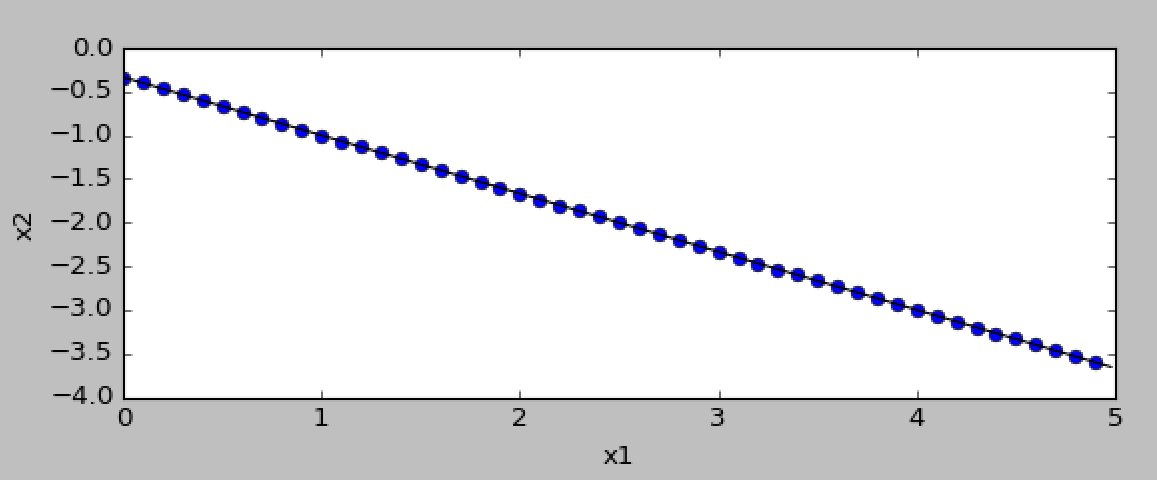
\includegraphics[scale=.5]{1-2-1.png}
		\item When $w = [-1, -2, -3]^T$ ($a = -2/3$, $b = -1/3$):
		\\ 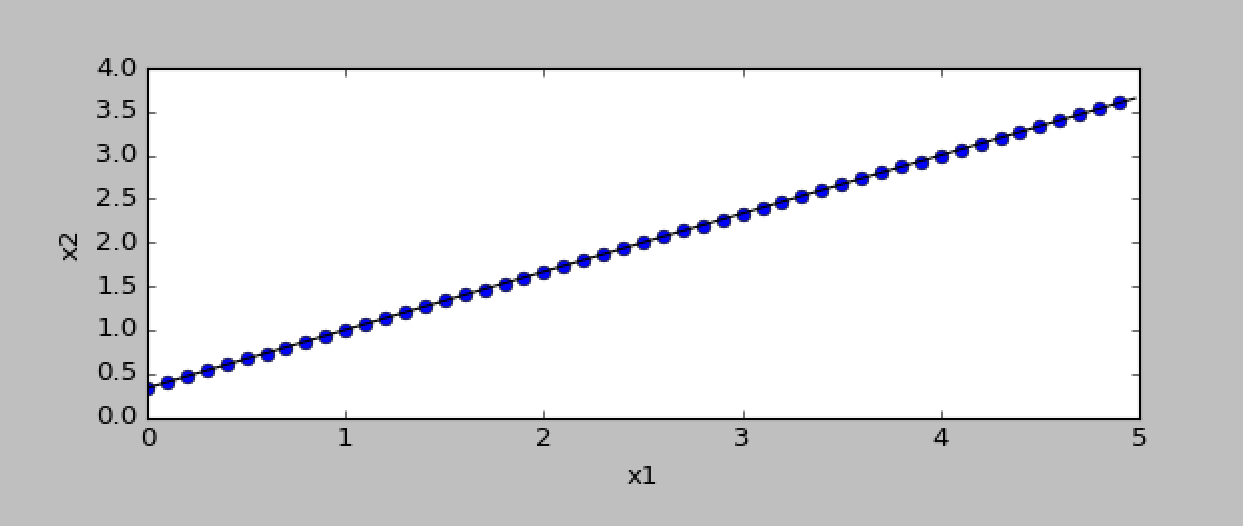
\includegraphics[scale=.5]{1-2-2.png}
	\end{enumerate}
\end{enumerate}

\section*{Problem 1.4}
\begin{enumerate}[label=(\alph*)]
	\item 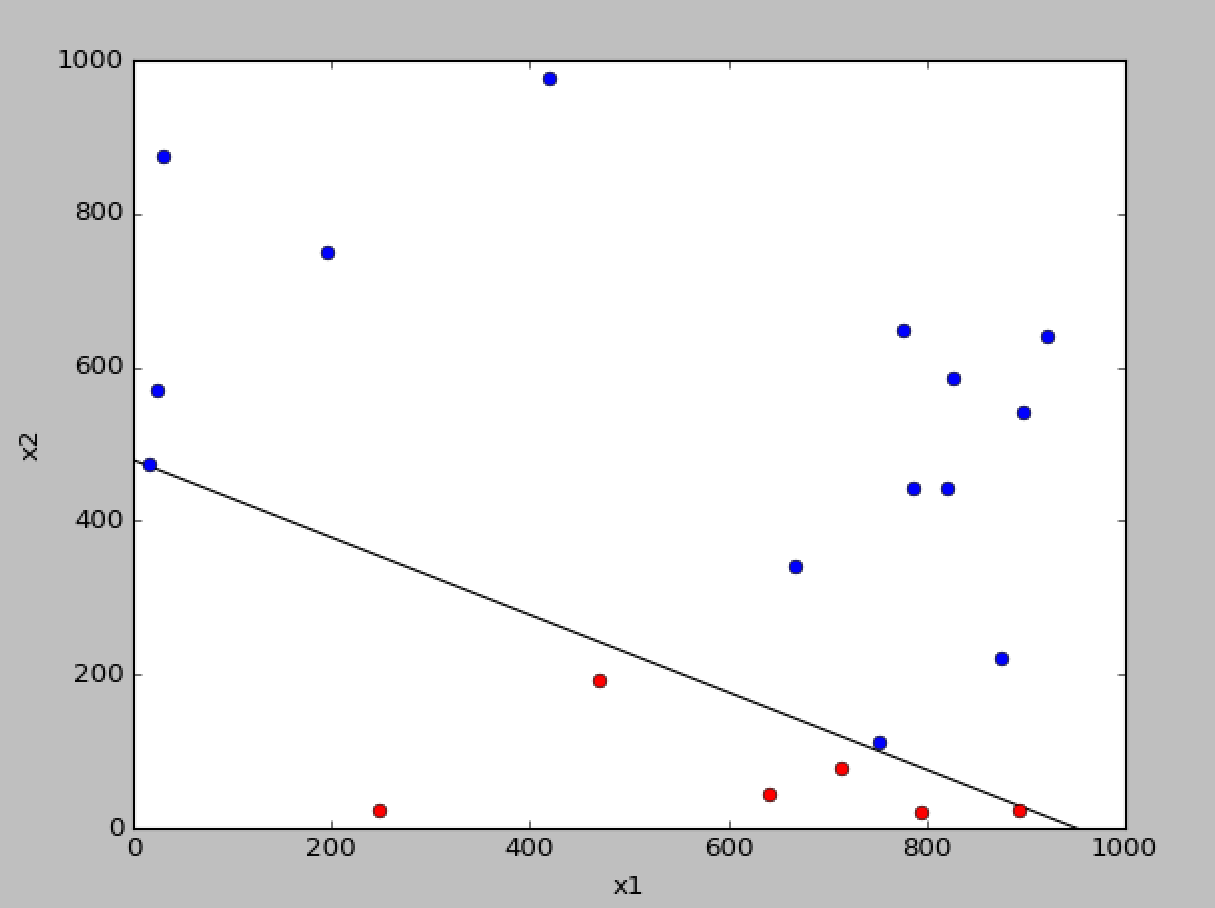
\includegraphics[scale=.5]{1-4-1.png}
	\item 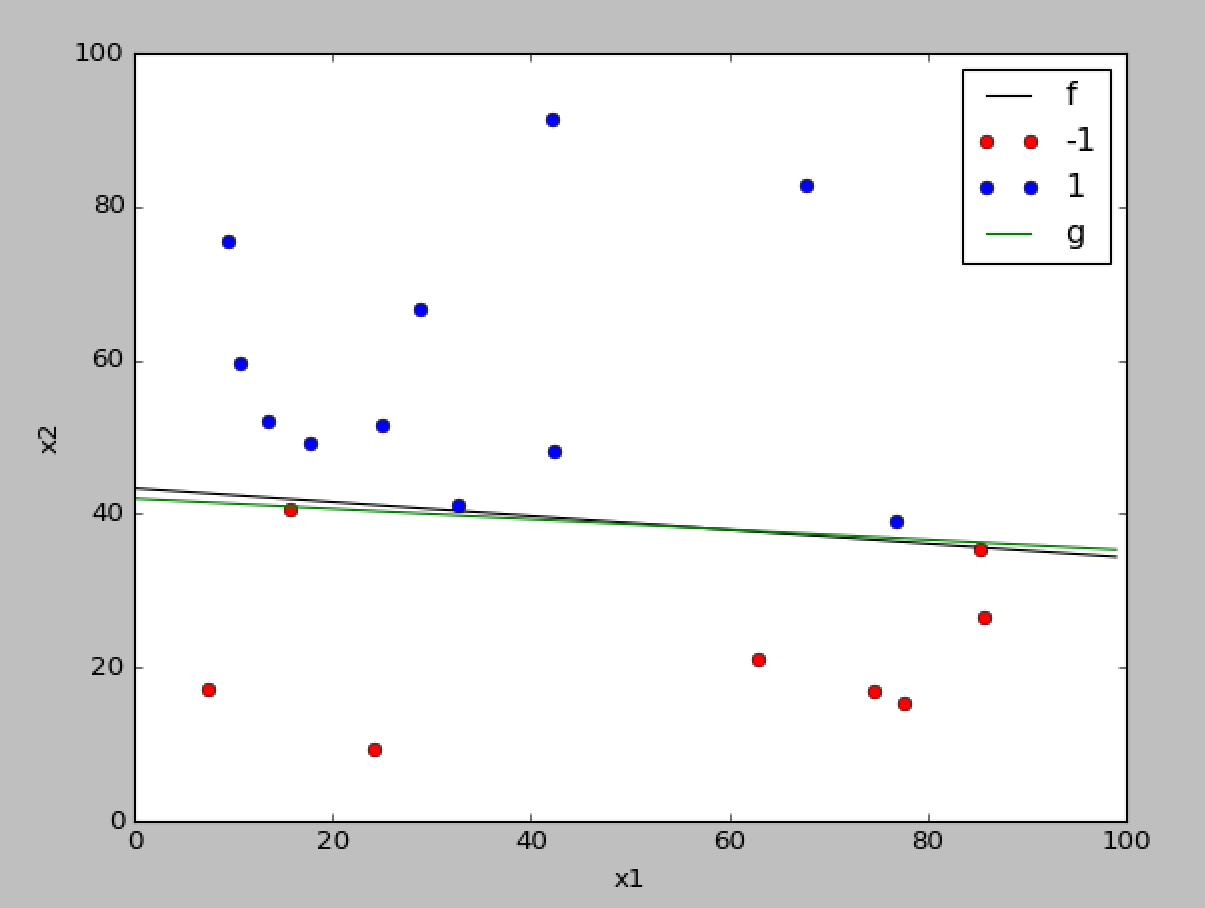
\includegraphics[scale=.5]{1-4-2.png}
	\\ 4699 iterations
	\\ $f(x) = -.09x + 43.37$
	\\ $g(x) = -.067x + 41.99$
	\\ In this example, f is quite close to g, due to the nature of the points (they tended to hug the line a lot)
	\item 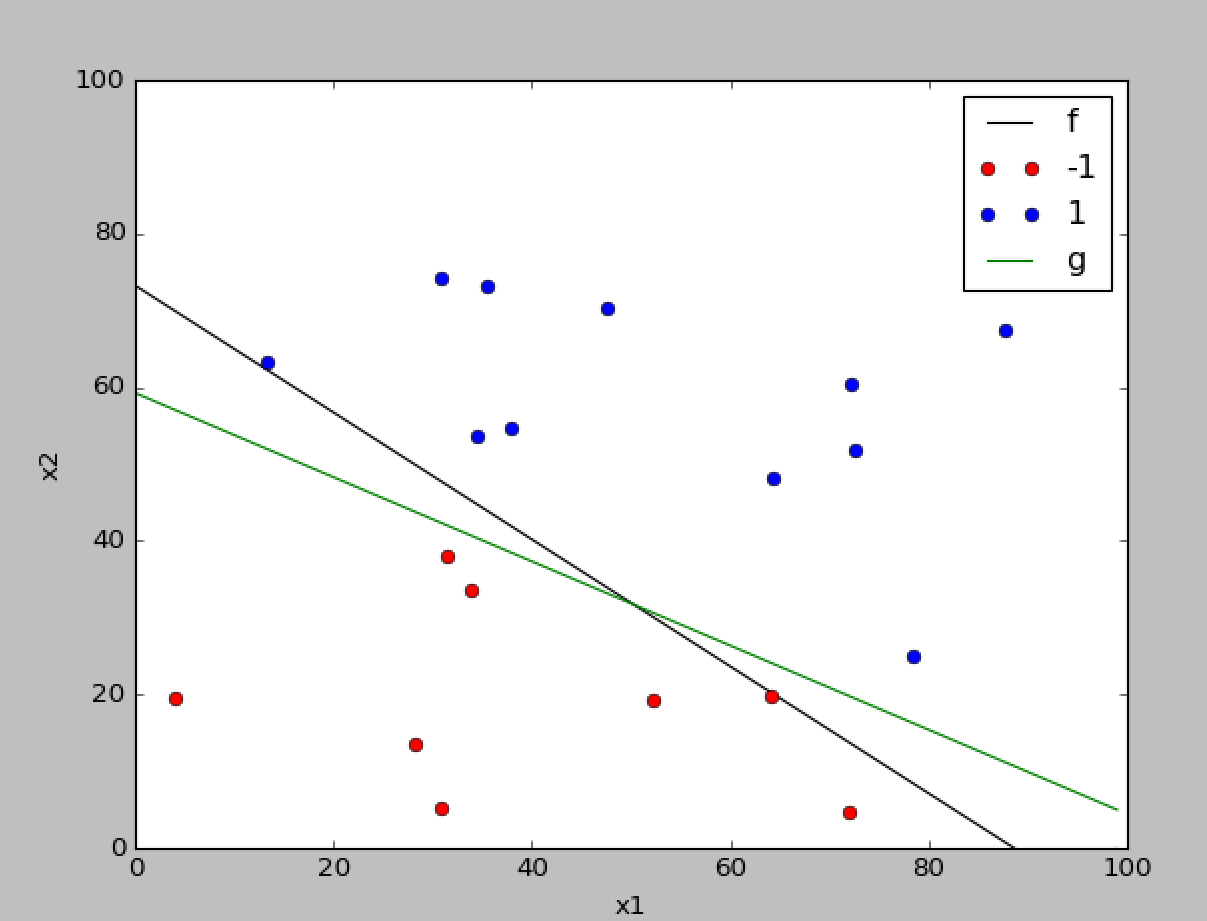
\includegraphics[scale=.5]{1-4-5.png}
	\\ 13112 iterations
	\\ $f(x) = -.82x + 73.26$
	\\ $g(x) = -.548x + 59.255$
	\\ f and g were a lot more volatile here, as is expected. PLA did not find the separator nearly as quickly this time too.
	\item 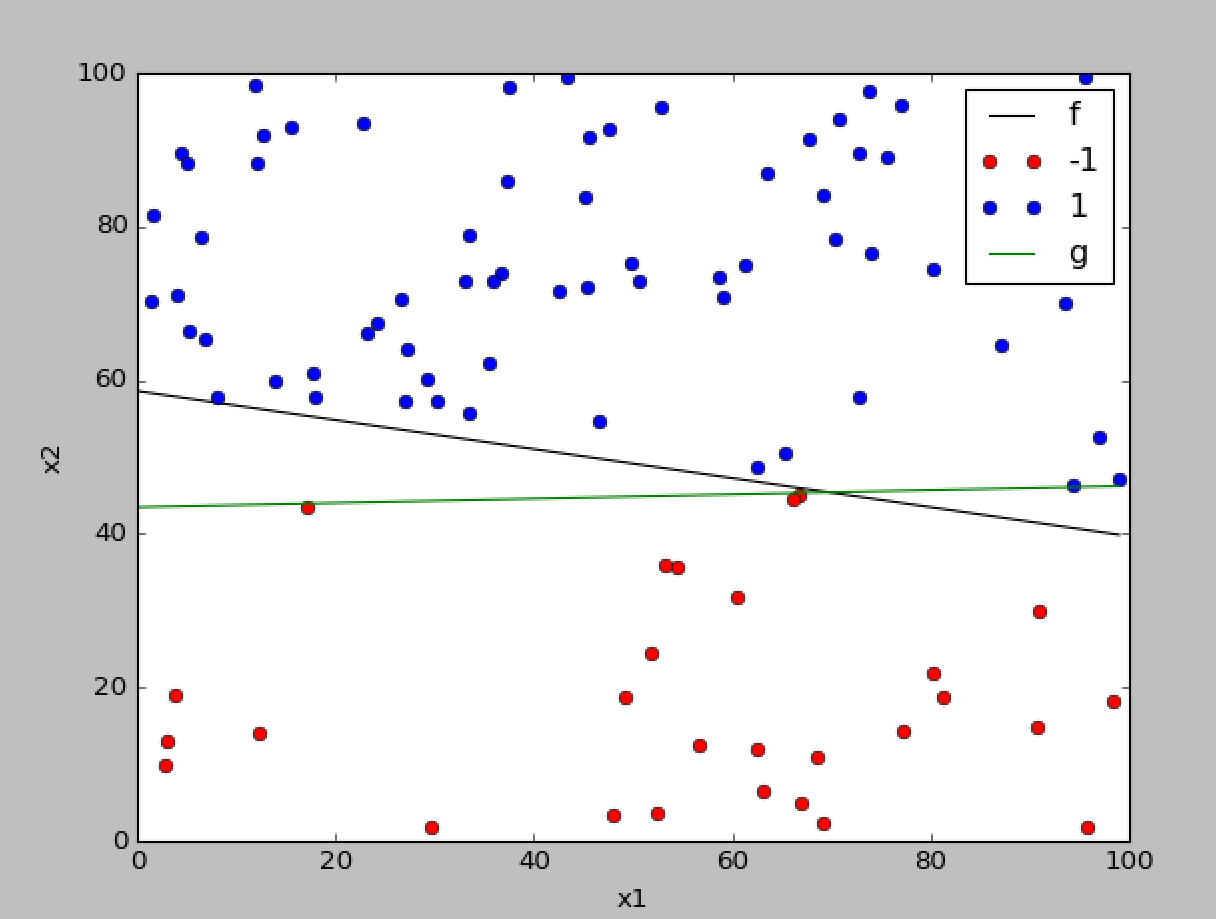
\includegraphics[scale=.5]{1-4-3.png}
	\\ 171142 iterations
	\\ $f(x) = -.18x + 58.59$
	\\ $g(x) = .027x + 43.46$
	\\ f and g are not so close again, this is probably due to the fact that many of the points are very far away from the curve.
	\item 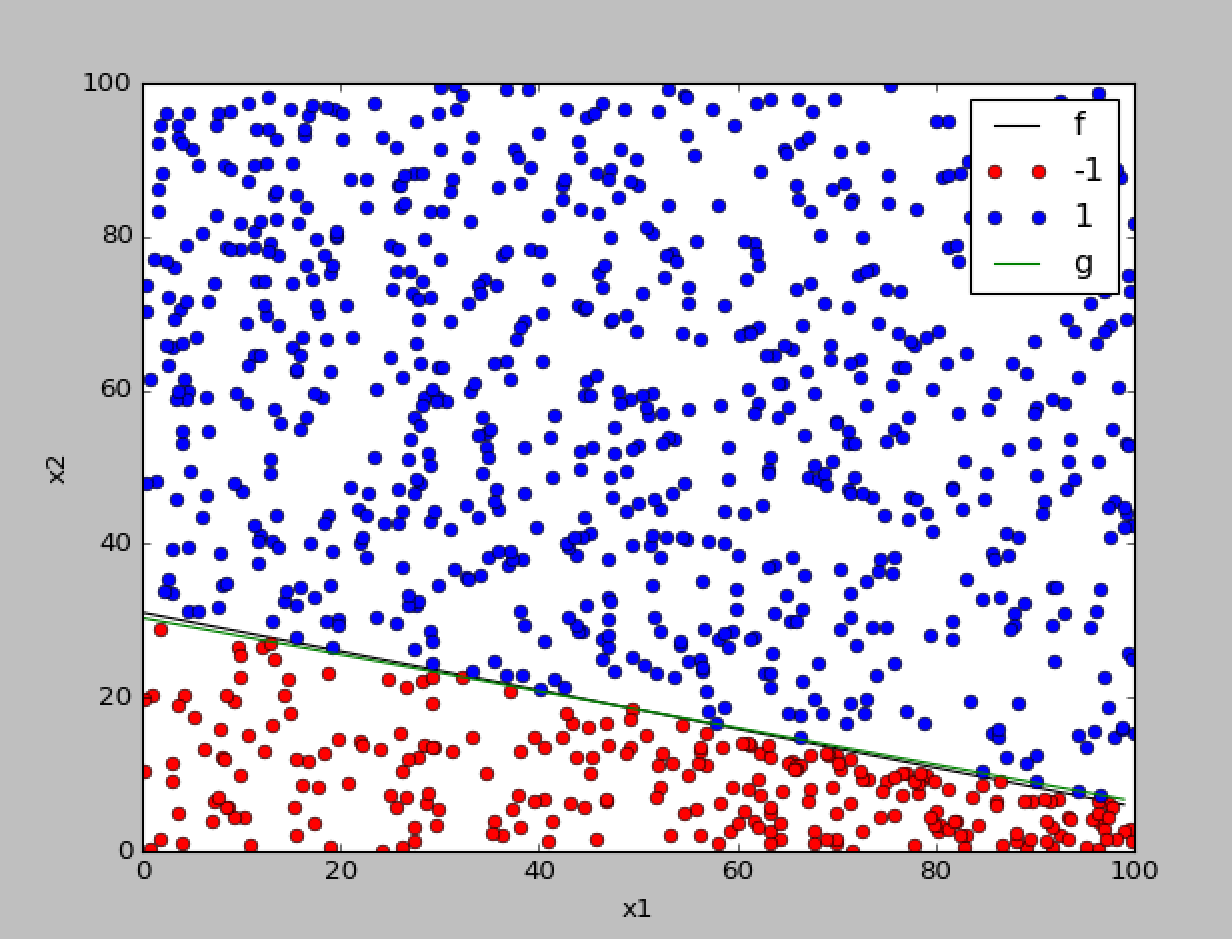
\includegraphics[scale=.5]{1-4-4.png}
	\\ 84205 iterations
	\\ $f(x) = -.25x + 31.05$
	\\ $g(x) = -.238x + 30.36$
	\\ f and g are practically identical. This is to be expected because of the sheer number of points.
\end{enumerate}

\end{document}